% Daniel: figure should take up the full width to be clearer to readers.
% \usepackage{subcaption}
% \begin{figure}[H]
% \begin{subfigure}{.25\textwidth}
%   \centering
%   % include first image
%   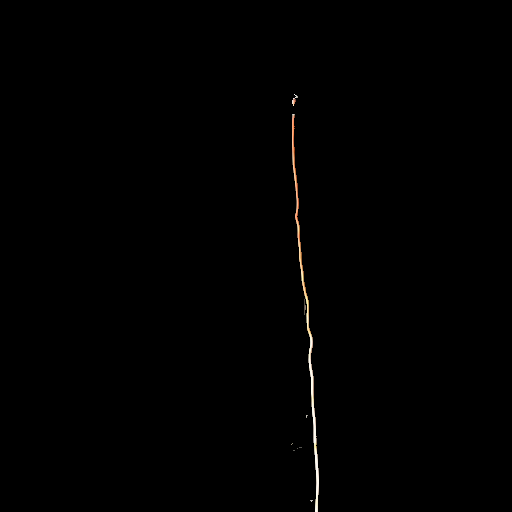
\includegraphics[width=.6\linewidth]{figures/taut_seg.png}  
%   \caption{Taut rope after reset}
%   \label{fig:sub-first}
% \end{subfigure}
% \begin{subfigure}{.25\textwidth}
%   \centering
%   % include second image
%   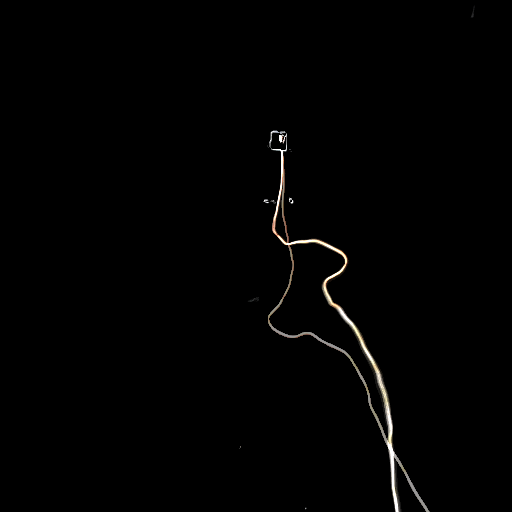
\includegraphics[width=.6\linewidth]{figures/repeat2.png}  
%   \caption{Repeatability across 20 trials}
%   \label{fig:sub-second}
% \end{subfigure}
% \caption{\textbf{Left: }the starting state of the rope is almost straight after being reset before each action begins. \textbf{Right: }overlaid image of 20 ending states of the rope after applying the same left-to-right whipping motion for 20 times given the same reset. The ending states of the rope are almost identical across 20 trials, with 1 outlier, so each action is repeatable. \harry{TODO: Re: Yes they are extremely similar. There is a kinda blurry region in the middle tho, and I did 10 more trials and had one outlier.} \jeffi{Random idea: Would it be possible to have each trial have a different color?  So we would see sort of  rainbow blob or cables?}}
% \label{fig:repeat}
% \end{figure}

\begin{figure}[t]
    \vspace*{5pt}
    \centering
    % \begin{tabular}{c@{\hspace{1.5pt}}c@{\hspace{1.5pt}}}
    %\subfloat[Ending states without reset]{%
    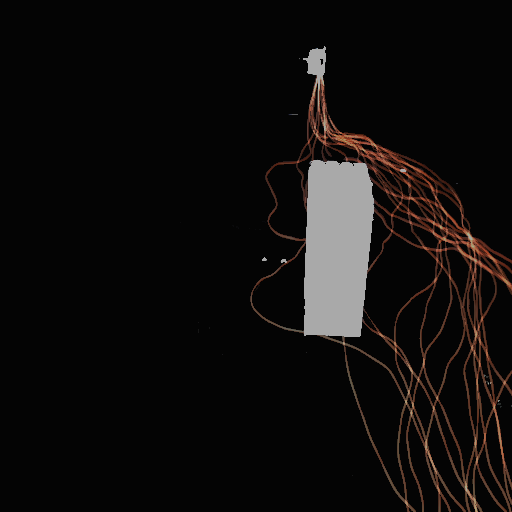
\includegraphics[height=122pt]{figures/unrepeata.png}%}%
    \hfill
    %\subfloat[Ending states with reset]{%
    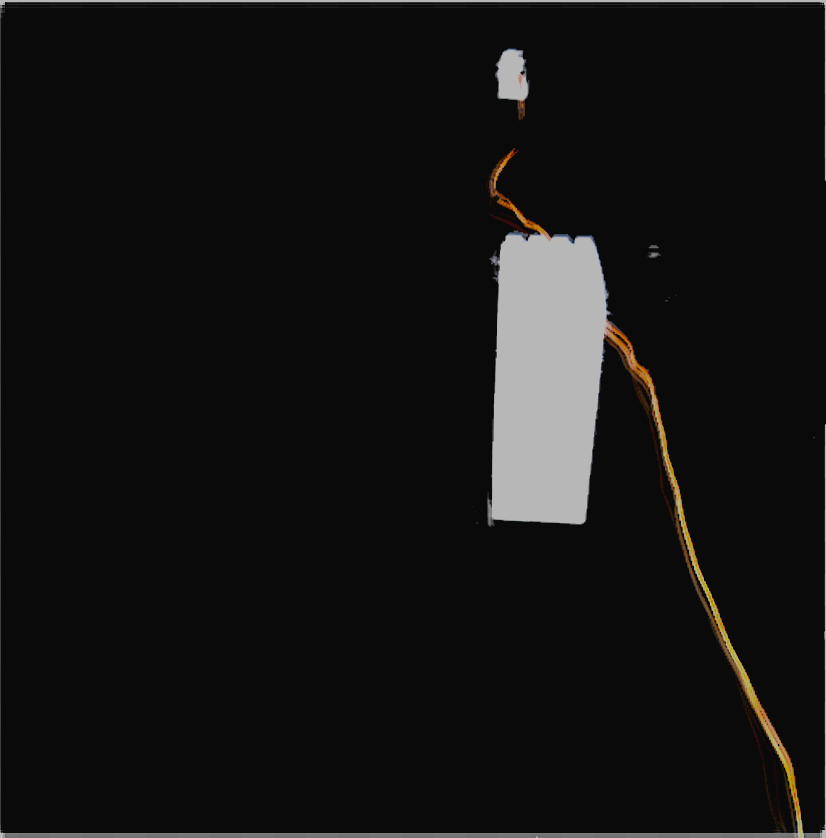
\includegraphics[height=122pt]{figures/repeat4a.png}%}
    % \end{tabular}
    \caption{\textbf{Repeatability without (left) and with (right) taut-pull reset.} 
    Both images show an overlay of 20 ending cable configurations after sequentially applying the same left-to-right vaulting trajectory 20 times. \textbf{Left: }without applying resets before the motion, there is high variation in ending configurations.  \textbf{Right: }resetting the cable via a taut-pull before the motion results in nearly identical configurations across 20 left-to-right attempts.}% The vaulting actions are surprisingly repeatable with reset.}
    %\vspace*{-10pt}
    \label{fig:repeat}
\end{figure}